\documentclass[oneside,a4paper,11pt,explicit]{book}
\usepackage[utf8]{inputenc}
\usepackage{icecream}
\usepackage[english]{babel}
\addto\captionsenglish{\renewcommand{\chaptername}{}}
\usepackage[accsupp]{axessibility}  % improves PDF readability for those with disabilities.
\usepackage[colorlinks = true,urlcolor  = blue,linkcolor = blue]{hyperref}
\usepackage{setspace}
\usepackage{listings}
\usepackage[most]{tcolorbox}
\usepackage{minitoc}
\usepackage{multicol}


\renewcommand{\mtifont}{\large\sffamily}
\renewcommand{\mtcfont}{\small\sffamily}
\renewcommand{\mtcSfont}{\small\sffamily}
\renewcommand{\mtcSSfont}{\small\sffamily}
\renewcommand{\mtcSSSfont}{\small\sffamily}
\mtcsetpagenumbers{minitoc}{off} % turn off page numbering in minitocs
\addto{\captionsenglish}{% Making babel aware of special titles
	\renewcommand{\mtctitle}{Quick Links To Sections}
}
\setlength{\fboxrule}{5pt}
\setlength{\fboxsep}{4pt}

\definecolor{IceCreamLeaf}{HTML}{58743b}
\definecolor{IceCreamOrbit}{HTML}{732e00}
\definecolor{MACred}{rgb}{0.803921568627451, 0.3607843137254902, 0.3607843137254902}

\title{I.C.E.C.R.E.A.M. Tutorials}
\subtitle{\small Observing Earth from Above (Env 329) v24.06  \\
	\small Schmid College of Science and Technology, Chapman University}
\date{\today}

%% DOCUMENT
\setstretch{1.25}
\makeatletter
\begin{document}

\setcounter{tocdepth}{3}
\setcounter{minitocdepth}{3}
\dominitoc
\faketableofcontents

\setcounter{chapter}{4} %Insert (Tutorial Number-1) Here; example for tutorial 4, enter 3

\chapter{Visualizing Data with QGIS} %Enter Tutorial Name Here

\vspace{-2em}

\minitoc

\hrule

\vspace{1em}

\begin{tcolorbox}[enhanced,frame style image=blueshade.png,
	opacityback=0.75,opacitybacktitle=0.25,
	colback=blue!5!white,colframe=blue!75!black,title={\Large \textbf{Objectives:}}]
	\large
	\begin{enumerate}
		\item Familiarize yourself with QGIS's toolbars, buttons, \& layout.
		\item Visualize land surface temperature data from ECOSTRESS in QGIS.
	\end{enumerate}
\end{tcolorbox}

\clearpage

%%%%%%%%%%%%%%%%%%%%%%%%%%%%%%%%%% Change Header to Have a Smaller Logo for Remainder of the Document
\fancyhead{}
\fancyhead[C]{\begin{tikzpicture}[overlay, remember picture]
		\fill[Blue2] (current page.north west) rectangle ($(current page.north east)+(0,-1in)$);
		\node[anchor=north west, text=white, font=\Large, minimum size=1in, inner xsep=5mm, align=left] at (current page.north west) {\bf{\MakeUppercase{\@title}}\\\@subtitle};
		\node[anchor=north east, minimum size=1in, inner xsep=5mm] at (current page.north east) {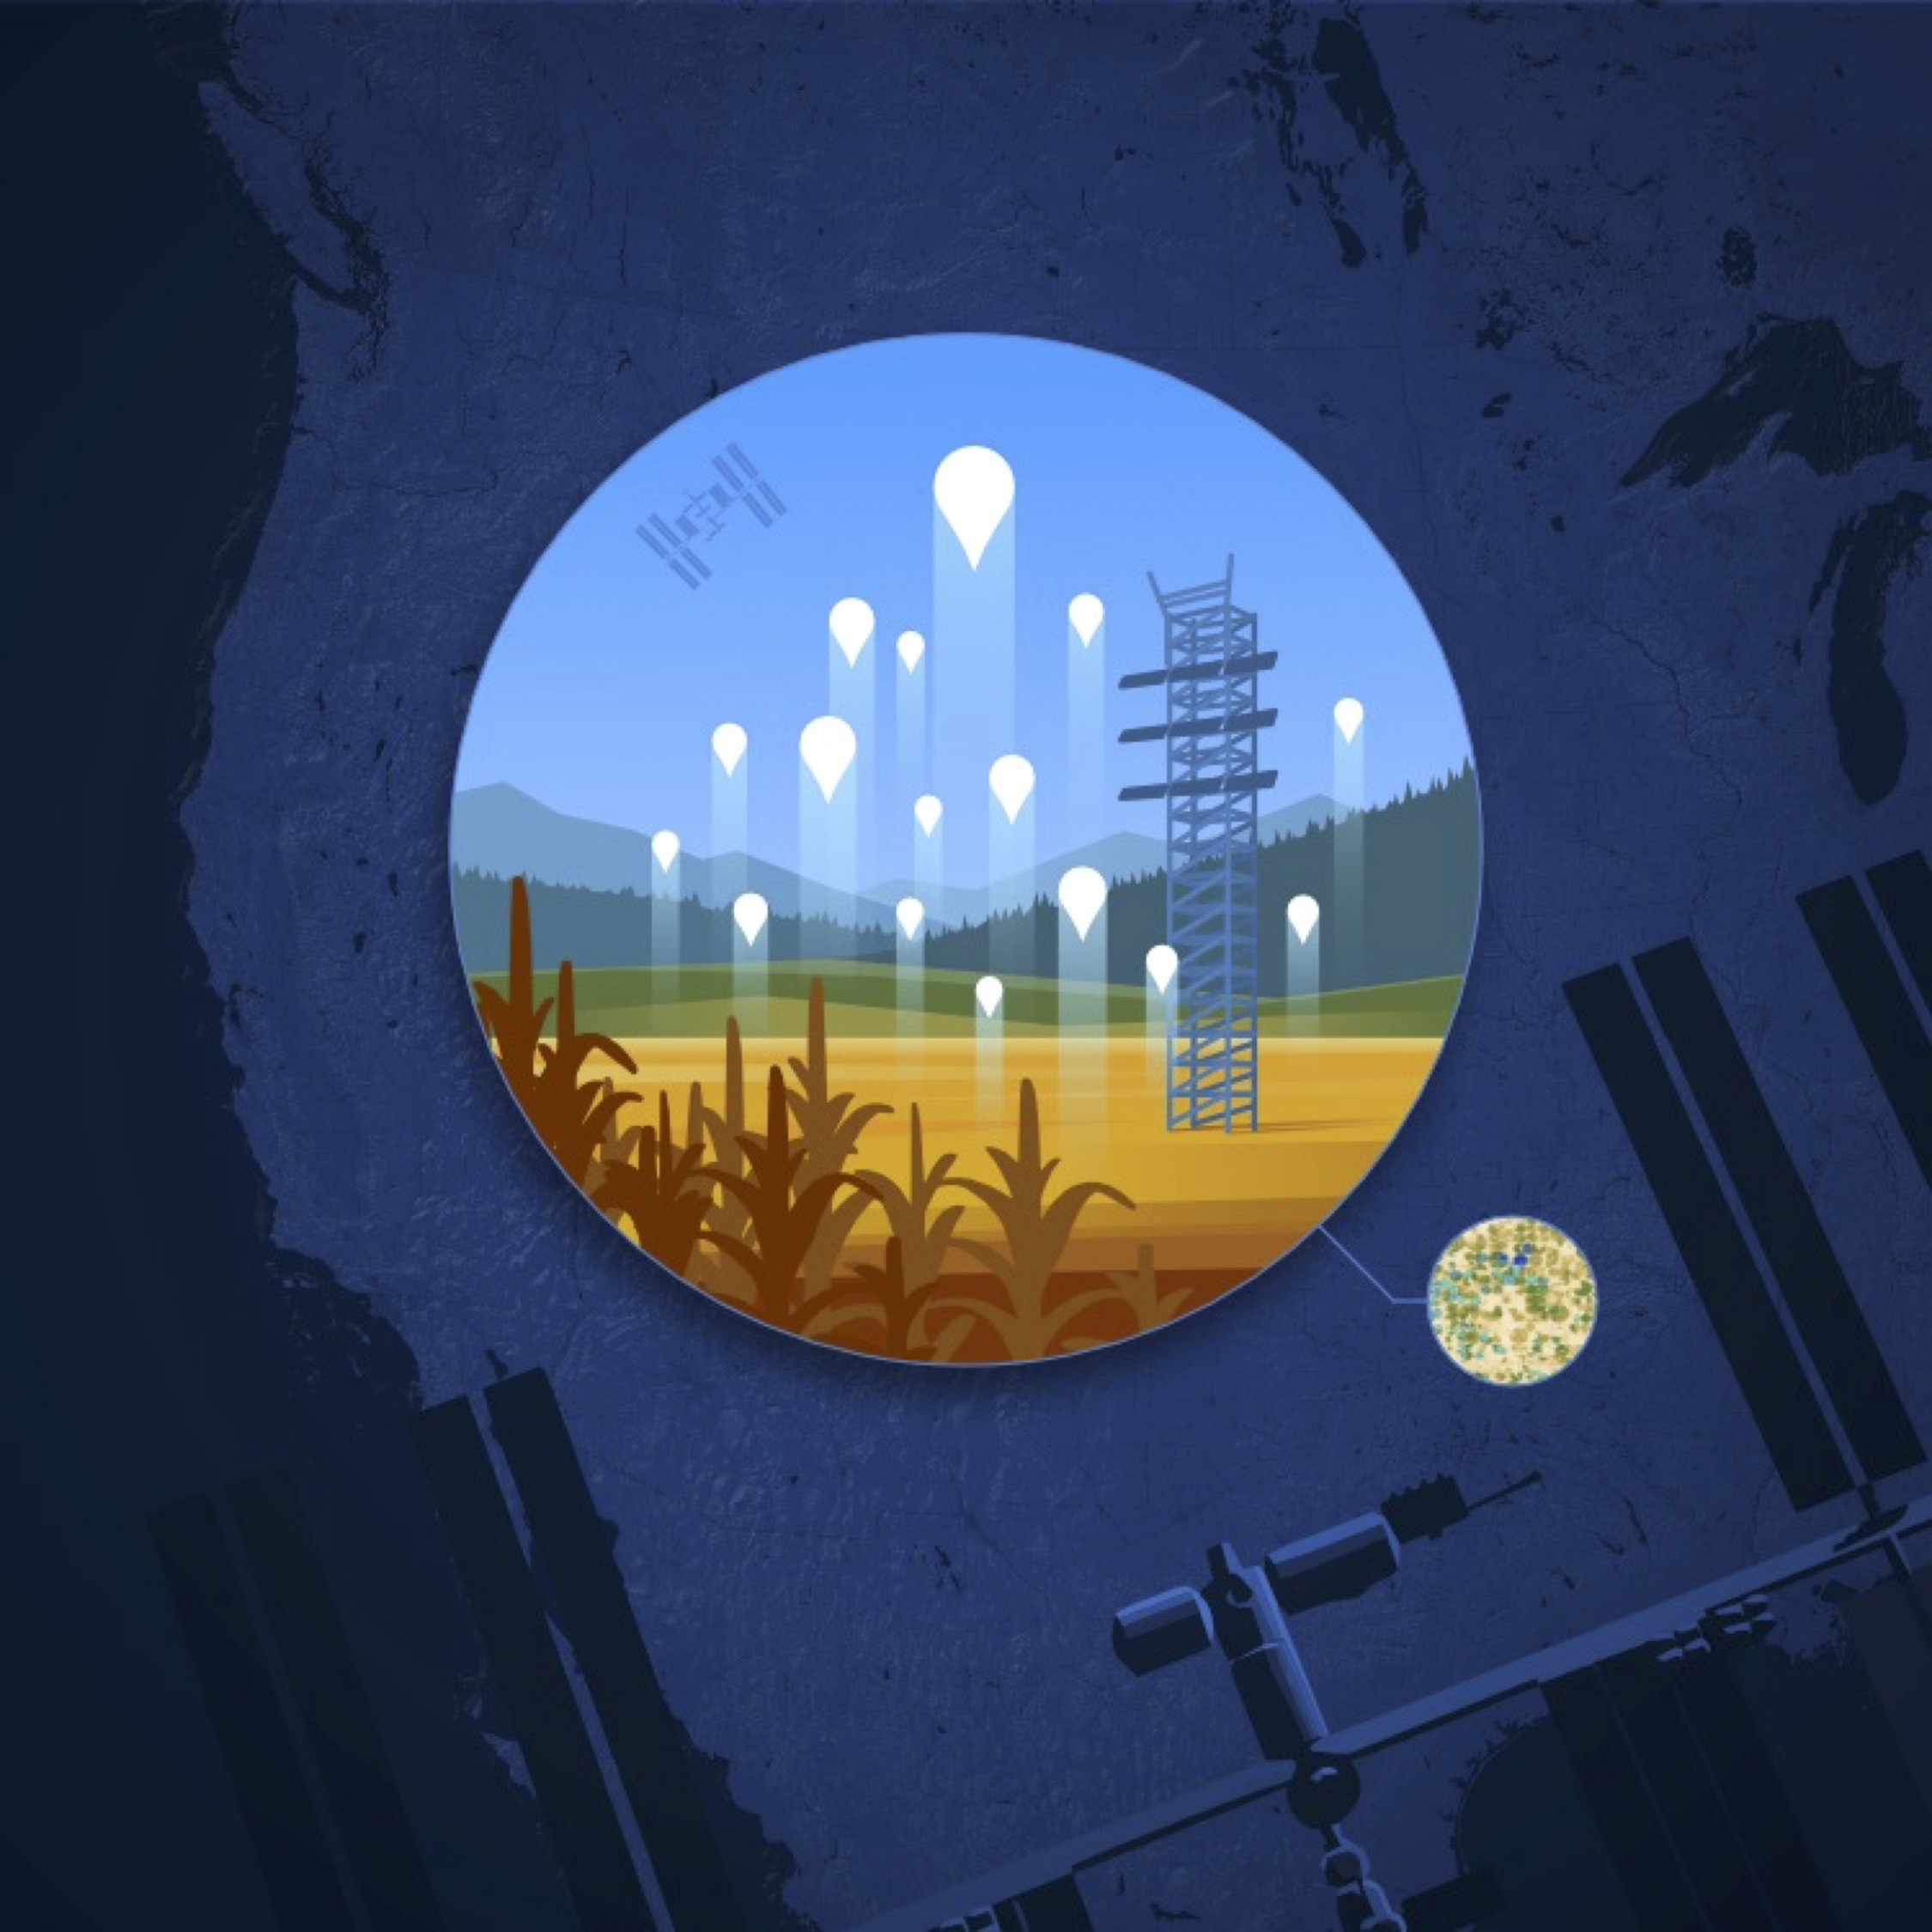
\includegraphics[scale=.03]{ECOSTRESS-BASE.jpg}};\end{tikzpicture}}
%%%%%%%%%%%%%%%%%%%%%%%%%%%%%%%%%%

\noindent\fbox{\begin{minipage}{.9665\textwidth}
			
	\vspace{1em}
	\begin{center}
		\textbf{\Large \underline{Motivation For Today's Tutorial: Heat in Death Valley}}
	\end{center}
	
	\addcontentsline{toc}{section}{Motivation : Death Valley}

	\vspace*{-1 em}
	
	\centerline{\includegraphics[width=\textwidth]{DeathValleySignECOSTRESS.png}}

	ECOSTRESS primarily measures land surface temperatures (LST), so let's look at the thermometer at one of the hottest places on the planet: Death Valley, California. The highest recorded ground temperature was verified at 201 °F on July 15, 1972. However, it recently had one of the hottest months on record, where air temperatures reached upwards of 128 °F in July of 2023. We are going to download the land surface temperature data from ECOSTRESS for those days to see how close it was to breaking the ground surface temperature record.
	
	\kulbox{\textbf{NOTE:} ECOSTRESS launched on July 9, 2018, so as you think about potential projects, you cannot design a project that requires data before that date.}

\end{minipage}}

\section{Basemaps \& Plugins}

In Tutorial 2, we used a simple basemap through a service included in the base QGIS installation. Today, we are going to expand QGIS's functionality by using another available \href{https://docs.qgis.org/3.28/en/docs/training_manual/qgis_plugins/fetching_plugins.html}{plugin}: HCMGIS. HCMGIS allows us to easily import basemaps from other services, such as ESRI, Bing, and Google.

\centerline{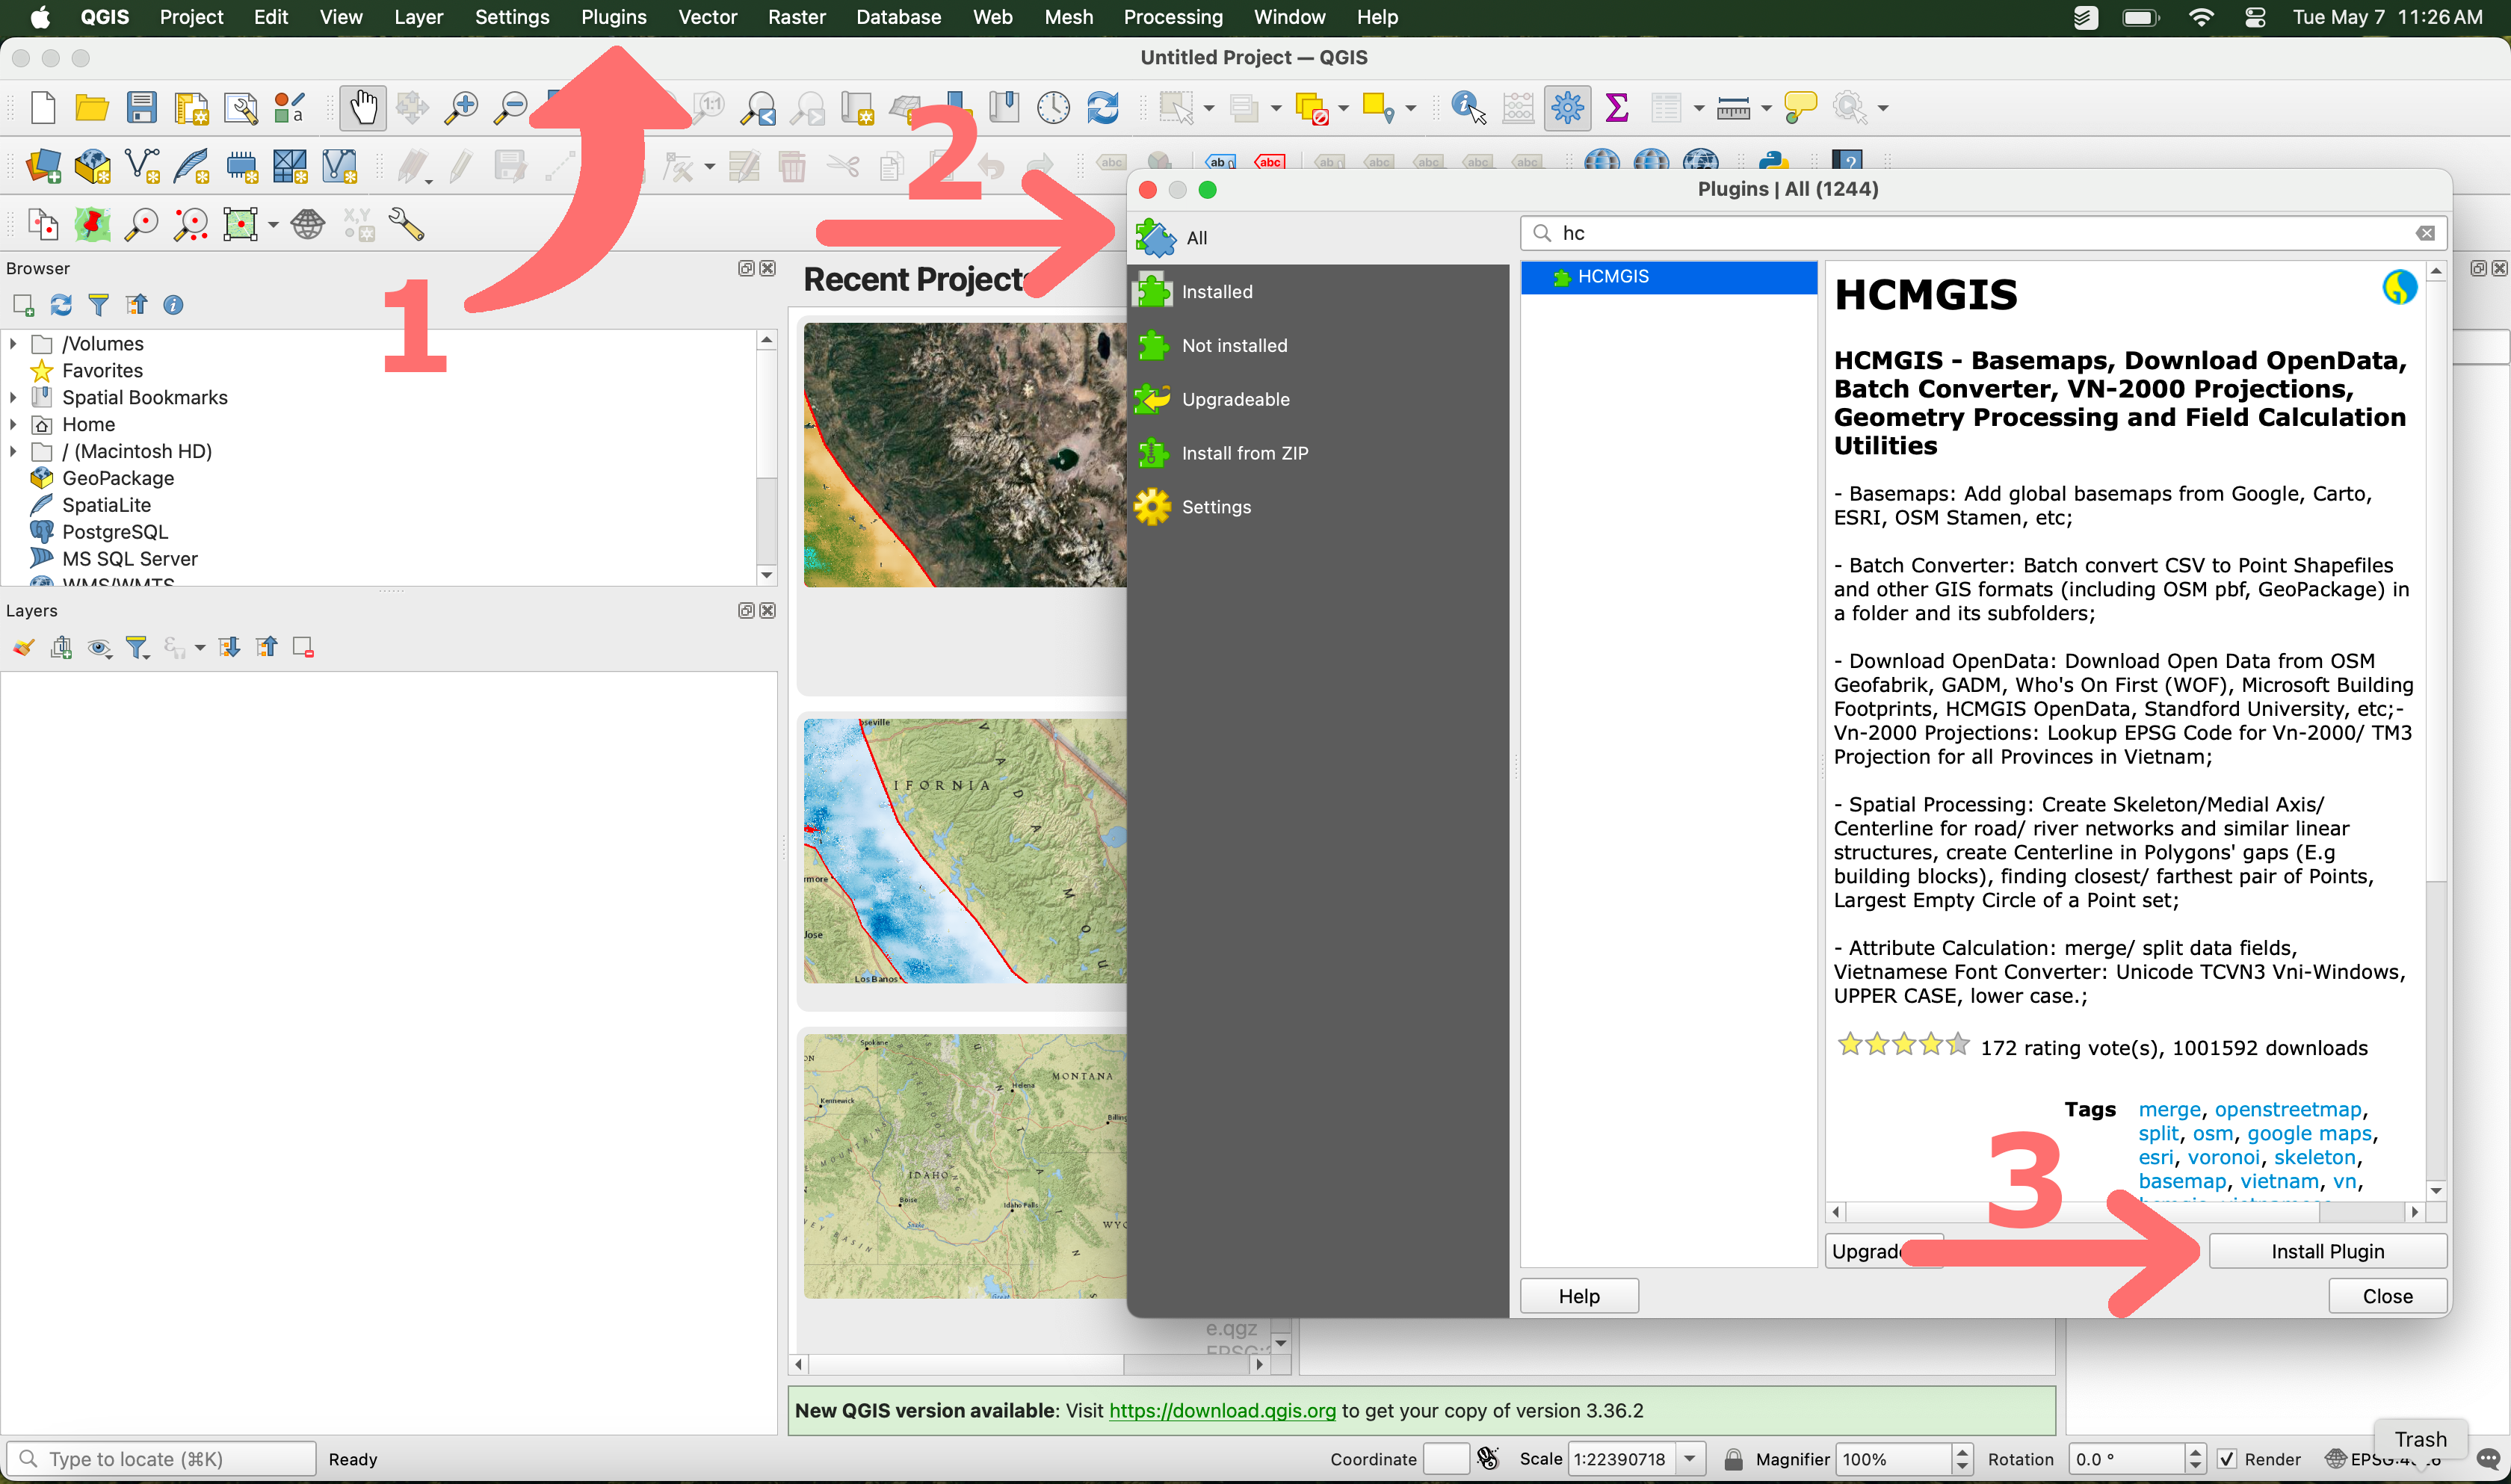
\includegraphics[width=\textwidth]{QGIS_Plugins.png}}

1. Open QGIS and start a new project by selecting the \textit{Project} menu $\rightarrow$ then \textit{New}. To install the HCMGIS plugin, click on the \textit{Plugins} drop down menu and select \textit{Manage and Install Plugins}.

2. In the next window, make sure \textit{All} is selected in the first window pane and search for HCMGIS. 

3. Click \textit{Install Plugin} and wait for the installation to complete.

\vspace{1em}

\centerline{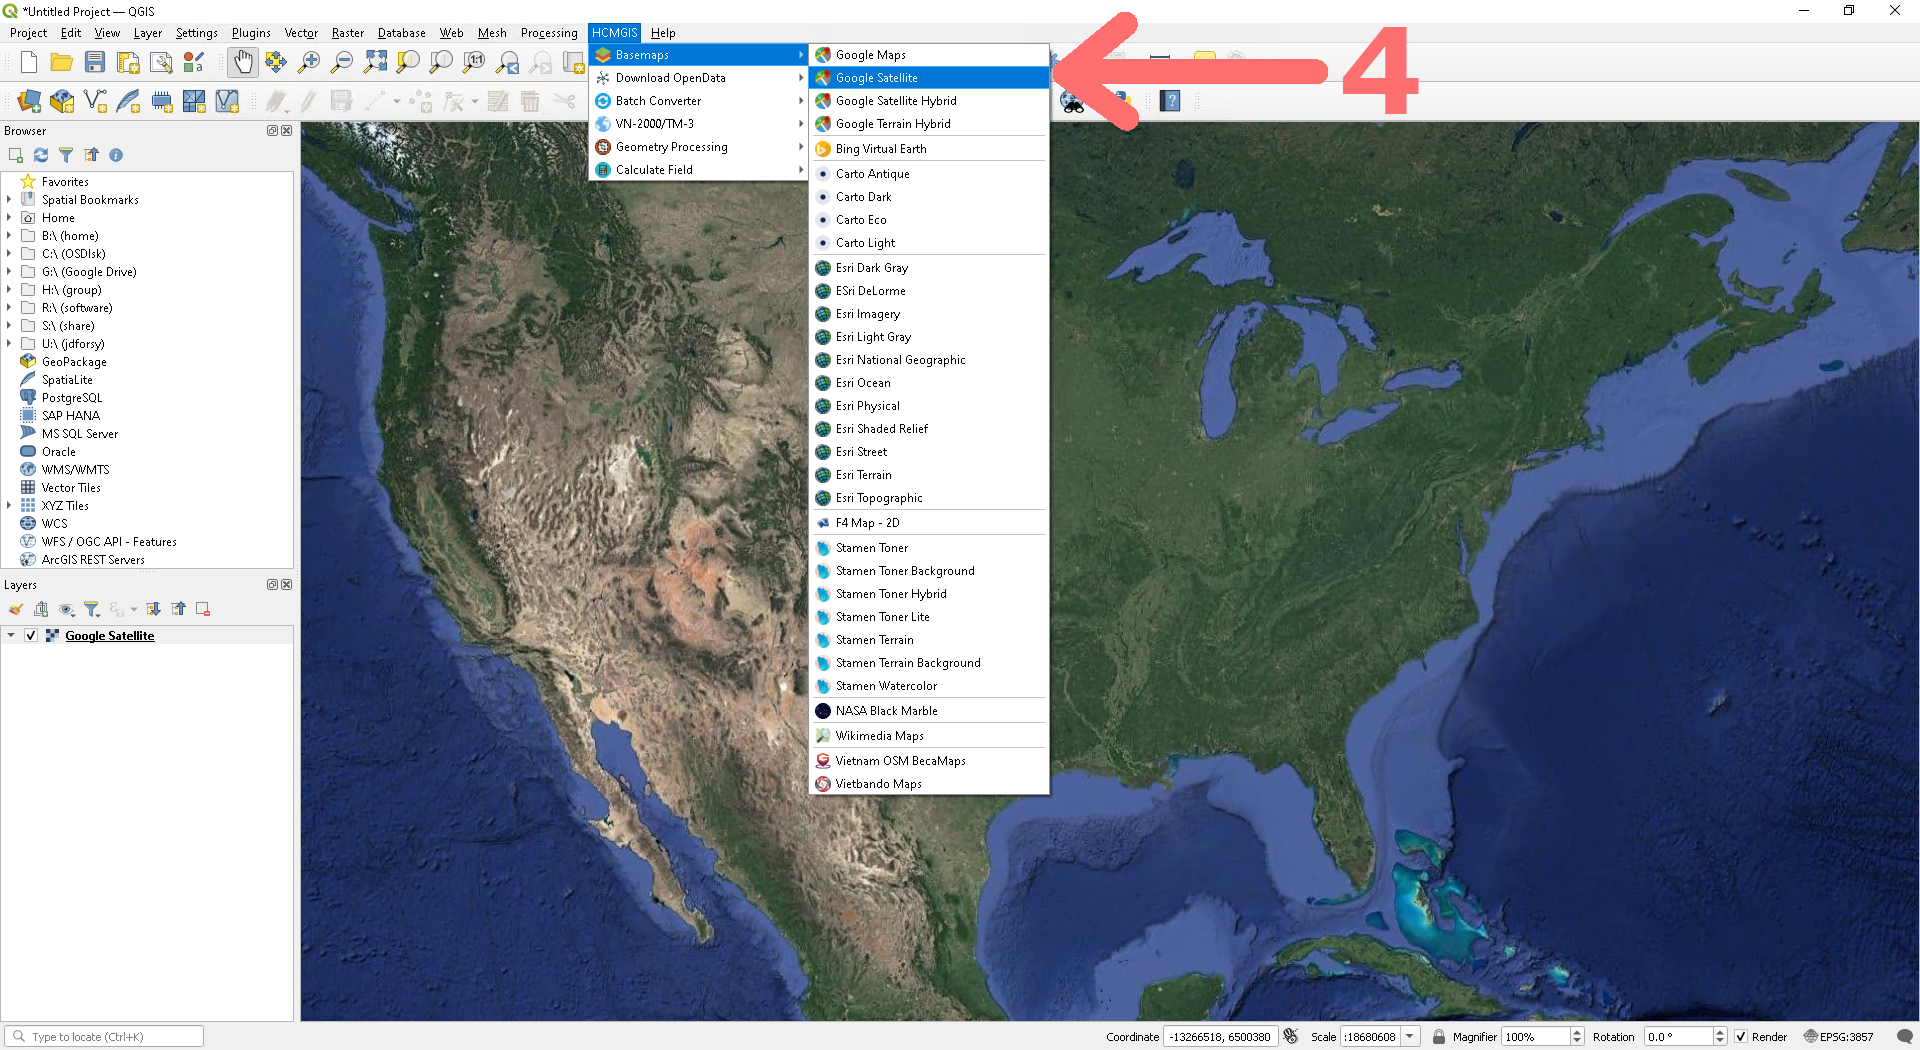
\includegraphics[width=\textwidth]{GoogleBasemap.png}}

\vspace{1em}

4. To quickly and easily add a basemap, all you need to do is find the \textit{HCMGIS} menu bar, select \textit{Basemap}, then pick your preferred map. For today's map, we will use \textit{Google Satellite}, though you could play around with other options. Some other favorites are ``ESRI Imagery,'' ``ESRI Delorme,'' ``Stamen Terrain,'' and ``NASA Black Marble,'' though their utility depends on the goal(s) of your map. Note that clicking on a basemap type automatically adds a new layer to your map, as seen in the layer browser window.

\section{Importing Our ECOSTRESS Death Valley Layer}

\vspace{1em}

\centerline{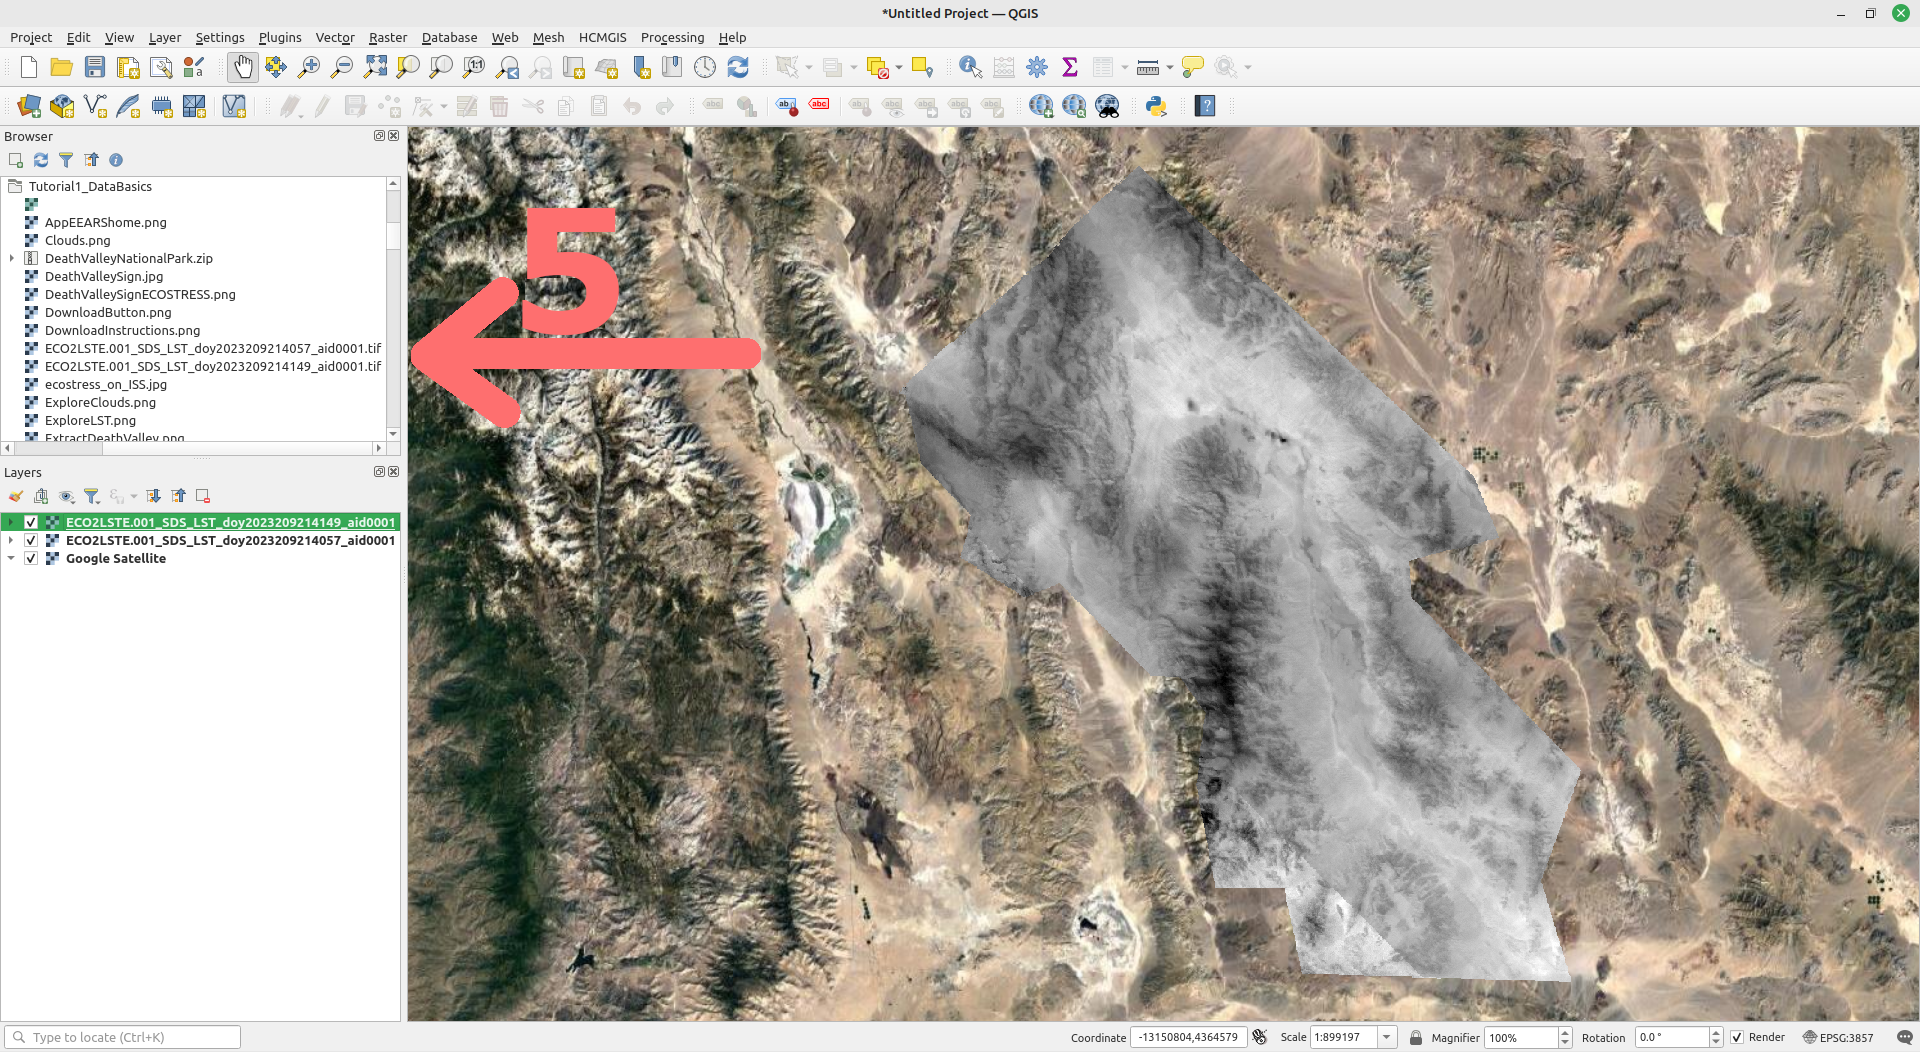
\includegraphics[width=\textwidth]{ImportLST.png}}

\vspace{1em}

5. Use the \textit{browser} window to find the folder where you saved the two Death Valley land surface temperature .tif files from tutorial 3. Double-click each file to add them to your map. Notice that they are now also listed in the \textit{Layers} window.

6. Congrats! You now have ECOSTRESS data on a map. But wait...let's make it look just a little better before you celebrate your win. QGIS doesn't know what kind of data this is and has defaulted to displaying the information in grayscale, which isn't that useful to our eyes. For each land surface temperature layer, right click on the layer name in the \textit{Layers} window and select \textit{Layer Properties}. On the menu bar to the left, select \textit{Symbology} and change the \textit{Render type} to Singleband pseudocolor. Since this is temperature, it is common to use a red color ramp. QGIS has automatically determined the minimum and maximum values from the datafiles; however, we have two files, so we need to match them. Specify 306.82 as the minimum and 347 as the maximum for both layers. Click \textit{apply}.

7. Finally, add the border from the DeathValleyNationalPark.zip shapefile. In the \textit{Browser} window, expand the zip file using the small arrow next to the filename. Double click on \textit{Death Valley National Park.shp} to add the layer. Right-click on the layer in the \textit{Layers} window and change the symbology to \textit{Outline
blue}. 


\kulbox{\textbf{NOTE:} You can also drag and drop the entire shapefile as a .zip into the \textit{Layers} window from an external file manager like \textit{Finder} on Mac or \textit{File Explorer} on Windows. This is sometimes useful when you have difficulty locating a file you have previously saved because you can use the search feature built into the file manager.}


\vspace{1em}

\centerline{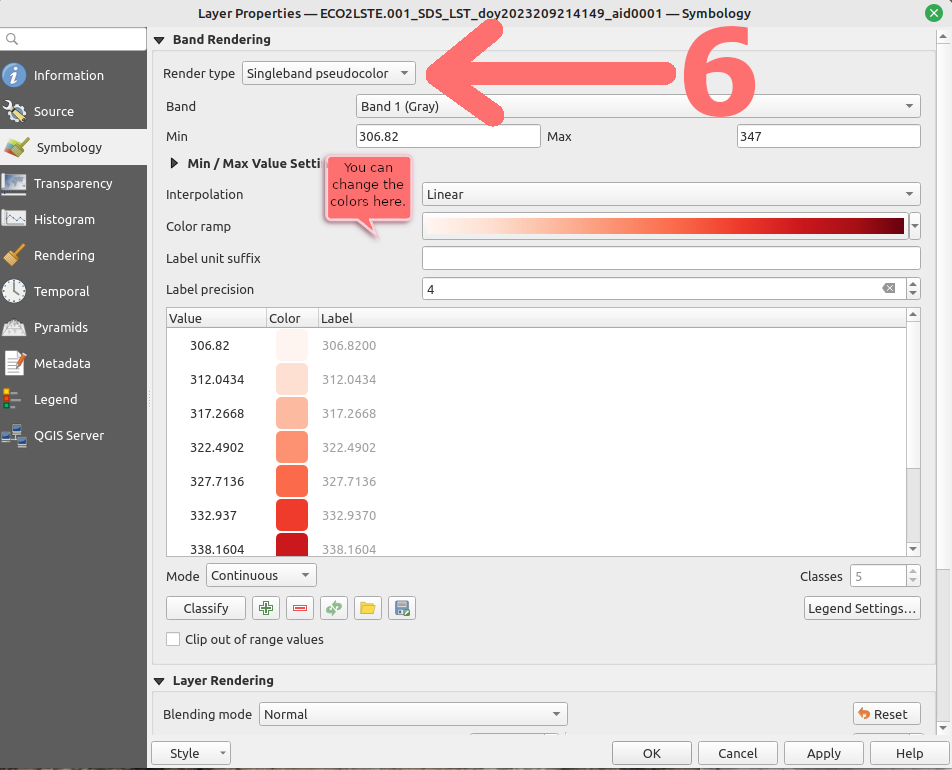
\includegraphics[width=.75\textwidth]{SymbologyLST.png}}

\vspace{1em}

8. Now we can celebrate! Your map should resemble the one below:

\vspace{1em}

\centerline{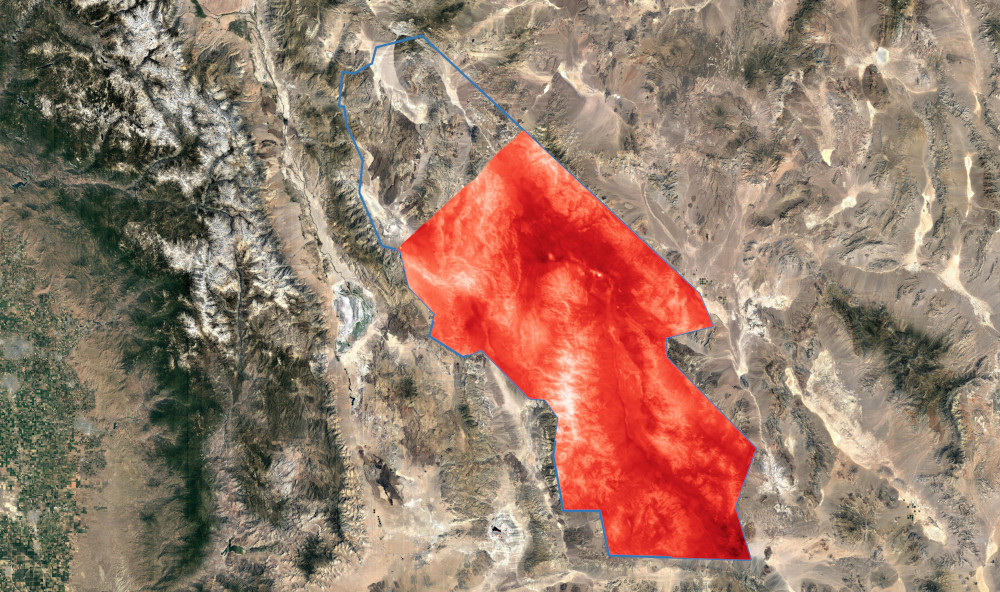
\includegraphics[width=\textwidth]{TempMap1}}

\vspace{1em}

\kulbox{\textbf{NOTE:} There was incomplete data coverage for the park, which is why the northernmost part  does not have any color displayed. This happens sometimes due to the orbit of the satellite.}

\newpage

9. Save your QGIS Project to the folder with all of the other files from this tutorial by going to the \textit{Project} menu bar at the top and selecting \textit{Save As...}. Maintain the file format as .QGZ.

10. Finally, export your map. From the \textit{Project} menu, navigate to \textit{Import/Export} and select \textit{Export Map To Image}. Increase the resolution to 200 dots per inch (DPI). 

\vspace{1em}

\centerline{
\includegraphics[width=.25\textwidth]{high_five.png}}

\vspace{1em}

High Five! You have learned to download ECOSTRESS instrument data from A$\rho\rho$EEARS and make a basic map in QGIS.

\begin{tcolorbox}[colback=yellow!5!white,colframe=MACred,title= \vspace{.2em} \Large Make a Map Assignments]
	\addcontentsline{toc}{section}{Make a Map Assignments}
	\large
	\begin{enumerate}
  \item Watch the YouTube Videos:
\href{https://youtu.be/N-3zF10LbHg?si=HLST3CbIbDo_JuIR}{Vector vs. Raster Data}
and \href{https://youtu.be/N-3zF10LbHg?si=HLST3CbIbDo_JuIR}{What is a Basemap}
  
  \item  Use the polygon you developed for your hometown to download ECOSTRESS land surface temperature for the year 2023. It is possible that if you selected a very large geographic area for your polygon that the file size will exceed the AppEEARS file size limit. If this is the case, you could consider selecting a smaller area or submitting multiple requests.

  \item Once the data are available, determine the day with the hottest median temperature and the day with the coldest median temperature. 

  \item Download the geotifs with the data for the day with the hottest median temperature and the day with the coldest median temperature and save them somewhere appropriate. You will need the data to make your maps!

  \item Submit a screenshot of the boxplot of data you viewed on AppEEARS.  
	\end{enumerate}
\end{tcolorbox}

\begin{tcolorbox}[colback=yellow!5!white,title=\textbf{Datafiles}]
	\addcontentsline{toc}{section}{Datafiles}
	\large
	In case you encountered any issues with the A$\rho\rho$EEARS database, here are copies of the ECOSTRESS GeoTIFF files for Death Valley:
	\begin{enumerate}
		\item \href{https://jeremydforsythe.github.io/icecream-tutorials/Tutorial5_AccessingRemoteSensingDataWithAppears/ECO2LSTE.001_SDS_LST_doy2023209214149_aid0001.tif}{\small ECO2LSTE.001\textunderscore SDS\textunderscore LST\textunderscore doy2023209214149\textunderscore aid0001.tif}
		\item \href{https://jeremydforsythe.github.io/icecream-tutorials/Tutorial5_AccessingRemoteSensingDataWithAppears/ECO2LSTE.001_SDS_LST_doy2023209214057_aid0001.tif}{\small ECO2LSTE.001\textunderscore SDS\textunderscore LST\textunderscore doy2023209214057\textunderscore aid0001.tif}
	\end{enumerate}
\end{tcolorbox}

%%%%%%%%%%%%%%%%%%%%%%%%%%%%%%%%%%%%%%%%%%%%%%%%%%%%%%%%%%%%%%%%%%%%%%%%%%%%%%%%%%% End of Document
\vfill

\hrule

\vspace{1em}

\small \textbf{Recommended Citation:} Forsythe, J.D., G.R. Goldsmith, and J.B. Fisher. 2023. Observing Earth from Above Tutorials. Chapman University. \url{https://jeremydforsythe.github.io/icecream-tutorials/}

\vspace{1em}

This work is supported by funding from NASA ECOSTRESS Mission Grant \#80NSSC23K0309 (I.C.E. C.R.E.A.M.: Integrating Communication of ECOSTRESS Into Community Research, Education, Applications, and Media) and is openly licensed via \href{https://creativecommons.org/licenses/by-nc/4.0/}{CC BY-NC}.

\end{document}
